%                                                                 aa.dem
% AA vers. 8.2, LaTeX class for Astronomy & Astrophysics
% demonstration file
%                                                       (c) EDP Sciences
%-----------------------------------------------------------------------
%
%\documentclass[referee]{aa} % for a referee version
%\documentclass[onecolumn]{aa} % for a paper on 1 column  
%\documentclass[longauth]{aa} % for the long lists of affiliations 
%\documentclass[rnote]{aa} % for the research notes
%\documentclass[letter]{aa} % for the letters 
%\documentclass[bibyear]{aa} % if the references are not structured 
% according to the author-year natbib style

%
\documentclass{aa}  

%
\usepackage{graphicx}
%%%%%%%%%%%%%%%%%%%%%%%%%%%%%%%%%%%%%%%%
\usepackage{txfonts}
%%%%%%%%%%%%%%%%%%%%%%%%%%%%%%%%%%%%%%%%
\usepackage{tabularx}
\usepackage{amsfonts}
\usepackage{bbold}
\usepackage{color}
\usepackage{transparent}
\usepackage{hyperref}
\usepackage{transparent}
\usepackage{rotating}
\usepackage{caption}
\usepackage{subcaption}

% Only include extra packages if you really need them. Common packages are:
\usepackage{graphicx}	% Including figure files
\usepackage{amsmath}	% Advanced maths commands
\usepackage{amssymb}	% Extra maths symbols
\usepackage{tablefootnote}
\usepackage[flushleft]{threeparttable}

\newcommand{\sgx}{SgXB\xspace}
\newcommand{\sfxt}{SFXT}
\newcommand{\sg}{Sg\xspace}
\newcommand{\co}{CO\xspace}
\newcommand*{\hmxb}{HMXB\@\xspace}
\newcommand*{\rlof}{RLOF\@\xspace}
\newcommand*{\ns}{NS\@\xspace}
\newcommand*{\eg}{e.g.\@\xspace}
\newcommand*{\ie}{i.e.\@\xspace}
\newcommand*{\aka}{a.k.a. \@\xspace}
\newcommand*\diff{\mathop{}\!\mathrm{d}}
\newcommand{\mystar}{{\fontfamily{lmr}\selectfont$\star$}}
\newcommand*{\msun}{$M_{\odot}$\@\xspace}

%\usepackage[options]{hyperref}
% To add links in your PDF file, use the package "hyperref"
% with options according to your LaTeX or PDFLaTeX drivers.
%
\begin{document} 


   \title{Formation of wind-capture disc in Supergiant X-ray binaries}

   \subtitle{Consequences for Vela X-1 and Cygnus X-1}

   \author{I. El Mellah
          \inst{1}
          \and
          A. A. C. Sander
          \inst{2}
          \and
          J. O. Sundqvist
          \inst{3}
          \and
          R. Keppens
          \inst{1}
          }

   \institute{Centre for mathematical Plasma Astrophysics, 
   			 Department of Mathematics, KU Leuven, 
   			 Celestijnenlaan 200B, B-3001 Leuven, Belgium\\
              \email{ileyk.elmellah@kuleuven.be}
         \and
             Institut f{\"u}r Physik und Astronomie, 
             Universit{\"a}t Potsdam, 
             Karl-Liebknecht-Str. 24/25, 14476 Potsdam, Germany
         \and
             KU Leuven, Instituut voor Sterrenkunde, 
             Celestijnenlaan 200D, B-3001 Leuven, Belgium
             }

   \date{Received ...; accepted ...}

% \abstract{}{}{}{}{} 
% 5 {} token are mandatory
 
  \abstract
  % context heading (optional)
  % {} leave it empty if necessary  
   {In Supergiant X-ray binaries (\sgx), a compact object captures a fraction of the intense wind from an O/B Sg companion star on a close orbit. Proxies exist to evaluate the efficiency of mass and angular momentum wind accretion but they depend so dramatically on the wind speed that within the theoretical and observational uncertainty ranges, they only bring loose constrains. Furthermore, they often bypass the impact of orbital and dissipative effects on the flow structure.
}
  % aims heading (mandatory)
   {We study the wind dynamics and in particular, the angular momentum it gains and carries as it is accreted. We aim at evaluating the conditions of the formation of a disc-like structure around the accretor and its observational consequences for \sgx. 
}
  % methods heading (mandatory)
   {We use recent results on the wind launching mechanism to compute ballistic wind streamlines in the three-dimensional co-rotating frame of a binary system, accounting for the gravitational and radiative influence of the compact companion. Once it enters the Roche lobe of the accretor, we solve the hydrodynamics equations and evaluate the impact of different cooling prescriptions on the flow.}
  % results heading (mandatory)
   {A shocked region forms around the accretor as the flow is beamed. For wind speeds of the order of the orbital speed, the shock is highly asymmetric compared to the axisymmetric bow shock obtained for a purely planar homogeneous inflow. Provided we enable cooling within the shocked region, the flow always circularizes for wind speeds slow enough.
}
  % conclusions heading (optional), leave it empty if necessary 
   {Although the donor star does not fill its Roche lobe, a realistic wind-launching representation can lead to a flow slow enough when it enters the Roche lobe of the accretor to be significantly beamed and bent by the orbital effects. The net angular momentum of the accreted flow is then large enough to form a persistent disc-like structure whose properties depend on the cooling mechanism.
}

   \keywords{accretion, accretion discs -- X-rays: binaries -- stars: neutron, supergiants, winds, outflows -- methods: numerical}

   \maketitle
%
%________________________________________________________________

\section{Introduction}

Most stars are found in multiple stellar systems, especially the high mass ones \citep{Duchene2013}. Among them, a significant fraction will undergo a phase of mass transfer which can seriously alter their subsequent evolution. New observational insights on the long \citep{Abbott2016a} and short term \citep{Grinberg2017} evolution of High Mass X-ray Binaries (\hmxb) has aroused the compelling need for a more comprehensive description of mass transfer via wind accretion. 

%The Roche lobe overflow (\rlof) mass transfer at stake in Low Mass X-ray Binaries has been extensively studied and built up appeal for a better understanding of the accretion disks formed in the process. They have proved to be fruitful landscapes for a wide scope of instabilities which enlighten our interpretations of the observed photometric and spectroscopic time-variability in these systems. However, observations and theoretical arguments tend to rule out the possibility of a stable \rlof mass transfer when the donor star is significantly heavier than the accretor, which is the case in most \hmxb. 

In Supergiant X-ray binaries (\sgx), a supergiant O/B donor star is orbited by a compact object, generally a neutron star (\ns), embedded in the stellar wind. O/B stars are known to loose mass at a rate up to several 10$^{-6}$M$_{\odot}\cdot$yr$^{-1}$ through a wind whose launching mechanism was first determined by \cite{Lucy1970} and \cite{Castor1975} : the resonant line absorption of UV photons by partly ionized metal ions provide the outer layers of the star with a net outwards momentum. As the flow accelerates, it keeps tapping previously untouched Doppler-shifted photons and can reach terminal speeds up to 2,000km$\cdot$s$^{-1}$. It is the gravitational capture of a fraction of this abundant line-driven wind by the compact companion which produces the X-ray luminosity we observe in \sgx, of the order of 10$^{35-37}$erg$\cdot$s$^{-1}$.

Until now, the mass and angular momentum accretion rates pertaining wind accretion have been evaluated based on the Bondi-Hoyle-Lyttleton model \citep[BHL, see][for a review]{Edgar:2004ip} : a planar supersonic flow is gravitationally deflected by the gravitational field of an accretor and an overdense tail is formed in its wake. The mass accretion rate turned out to be so sensitive to the relative speed of the flow with respect to the accretor that within the uncertainties and local variations in a massive-star wind, any realistic \sgx mass accretion rate can be reproduced. Furthermore, the axisymmetry of the BHL problem circumvented any discussion on the accretion of angular momentum. This assumption was first relaxed by \cite{Illarionov1975} and \cite{Shapiro1976} to assess the possibility of the formation of a wind-capture disc around compact accretors : they concluded that it was likelier for close binaries, where the star gets close to fill its Roche lobe, but that it was also highly dependent on the relative wind speed. This dependency is made even more crippling when one notices that in \sgx, the accretor lies within the region of acceleration of the flow, which prevents us from simply relying on the terminal speed of the wind.

In consequence, a fully consistent treatment of both the wind acceleration and its accretion by the compact object is required to avoid being left with the wind speed as a convenient but not constraining degree of freedom. \cite{Sander2017} computed the steady state wind stratification for a 1D radial non-local thermal equilibrium atmosphere of a star representative of the donor star in Vela X-1. They accounted for a plethora of chemical elements and ionization levels susceptible to absorb the stellar UV photons, and for the X-ray ionizing feedback from the accretor on the wind ionization state. In this paper, we intend to use this computed 1D line-driven acceleration to see how the 3D structure of the flow departs from a spherical wind once the orbital effects are added. Rather than being set based on an empirical fitting formula, the static wind velocity and density are mere consequences of the stellar and orbital properties. In section\,\ref{sec:orb_dev}, we evaluate the systematic bending of the wind streamlines by the orbital effects, as the wind unfolds and enters the Roche lobe of the accretor with a non-zero net angular momentum. Within the latter, we run 3D HD simulations described in section\,\ref{sec:wind-capt_discs} to capture the structure of the flow as it cools down downstream the shock and its capacity to form a disc-like structure. In section\,\ref{sec:obs_cons}, the implications of such a component are discussed in the context of the archetype of wind accreting \ns-\sgx, Vela X-1, and of the \sgx Cygnus X-1 hosting a stellar-mass black hole candidate accreting the wind from a companion supergiant which does not fill its Roche lobe. 

%- - -
%
%Yet, we still miss a fully consistent frame to follow the flow from the stellar surface down to the X-ray emitting region, in the immediate vicinity of the accretor. Until now, the six orders-of-magnitude or so separating the two scales has precluded any bold numerical attempt to follow the flow all along its journey.
%
%\cite{Hoyle:1939fl} first derived a critical impact parameter, the accretion radius, below which material is likely to be captured by the accretor.
%
%brought a firm motivation
%
%brought serious motivations to the field of accretion disks
%
%The turbulent twilight of massive stellar binaries stars determines their final fate. In Supergiant X-ray binaries, mass transfer proceeds through the accretion of a fraction of the dense and fast wind from an evolved donor star by an orbiting compact object, generally a neutron star. The accretor both perturbs the stellar wind and provides a moving X-ray source to probe its internal structure : the characteristics of the flow constrain the X-ray emission and absorption along the line-of-sight, while the X-ray ionizing feedback alters the wind acceleration. In order to consistently monitor the flow from the stellar surface down to the accretor, we designed a multi-scale model which includes recent insights on the properties of massive star winds. We performed 3D numerical simulations to evaluate the mass and angular momentum accretion rates onto the compact object, depending on the wind to orbital speed ratio and to the cooling efficiency within the shocked region. We identified conditions favorable to the formation of a disc-like structure beyond the neutron star magnetosphere, in spite of the low angular momentum carried by the wind, and analyzed its properties. These conditions, compatible with the currently known parameters of the Supergiant X-ray binary Vela X-1 and to a certain extent with Cygnus X-1, indicate the possible presence of a limited disc-structure in the former case and account for an extended one in the latter case.
%
%
%Our current theories of single-star evolution have proved consistent with the observational surveys carried on by contemporary missions. However, few stars are deprived of a gravitationally bound stellar companion, with more high mass stars showing a higher multiplicity frequency \citep{Duchene2013}. Some of them undergo a phase of interaction with their companion tied enough to significantly alter their subsequent evolution. One of the stages important to provide a more complete evaluation of the impact of binarity on stellar evolution are high mass X-ray binaries (\hmxb). They represent the turbulent twilight of the entangled evolution of two massive stars, one having already collapsed into a compact object. They are believed to be progenitors of compact object binaries whose final coalescence has been observed by the LIGO/VIRGO collaboration \citep{Abbott2016a}.
%
%The main characteristic manifestation of binarity is through mass transfer between the two components. It can lead to chemical contamination \citep[\eg in the case of Barium and Carbon-enhanced metal-poor stars][]{Boffin2014,Masseron2009} or to the stripping of the outer envelope of an evolved star, leaving a naked Helium-rich core \citep[\eg for some hot subdwarf stars][]{XXX Podsiadlowski2010, Mereghetti2014 or Han? XXX}. The transfer of mass goes hand in hand with a transfer of angular momentum which can produce fast rotators like millisecond pulsars \citep{XXX Podsiadlowski2010? XXX} or Be-stars \citep{XXX Podsiadlowski2010? XXX}.
%
%Supergiant X-ray Binaries (\sgx) are systems where a compact object, generally a neutron star, orbits an O/B Supergiant \citep[see][for a recent review]{Martinez-Nunez2017}. Mass transfer proceeds through the capture of a fraction of the dense and fast line-driven stellar wind by the accreting body. This highly non-conservative mechanism, called wind accretion, has been put in opposition to the better understood Roche lobe overflow mechanism, although elements of both can co-exist in hybrid models \citep{Mohamed,ElMellah2016a}. The central distinction lies in the presence of a large and permanent disc in the latter case, while the conditions for such a structure in the former case are still unclear. Our present knowledge on angular momentum wind accretion builds up on models of asymmetric Bondi-Hoyle-Lyttleton accretion \citep{Illarionov1975,Shapiro1976} and on numerical investigations of the impact of transverse gradients of density \citep{Ruffert1999,MacLeod2015} and velocity \citep{Ruffert1996}. Yet, we still miss a fully consistent frame to follow the flow from the stellar surface down to the X-ray emitting region, in the immediate vicinity of the accretor. Until now, the six orders-of-magnitude or so separating the two scales has precluded any bold numerical attempt to follow the flow all along its journey.
%
%Wind accretion turns out to be extremely sensitive to the properties of the stellar wind. O/B supergiants display dense and fast outflows, with mass loss rates up to several solar masses per million year. The underlying mechanism, unveiled by \cite{Lucy1970} and \cite{Castor1975}, is the resonant line absorption of UV photons by partly ionized metal ions in the outer layers of the star. As the flow accelerates, it keeps tapping previously untouched Doppler-shifted photons XXX FOR ANDREAS : INFLUENCE OF DETAILED IONIZATION STRUCTURE AND X-RAY IONIZING FEEDBACK XXX
%
%
% key-ingredient


% ------------------------------------------------
\section{Orbital deviation of the wind}
\label{sec:orb_dev}
% ------------------------------------------------

% - - - - - - - - - - - - - - - - - - - - - - - - 
\subsection{Model and numerical method}
\label{sec:orb_model}
% - - - - - - - - - - - - - - - - - - - - - - - - 
%(and neglect Roche deformation of the star)

%\begin{figure}
%\centering
%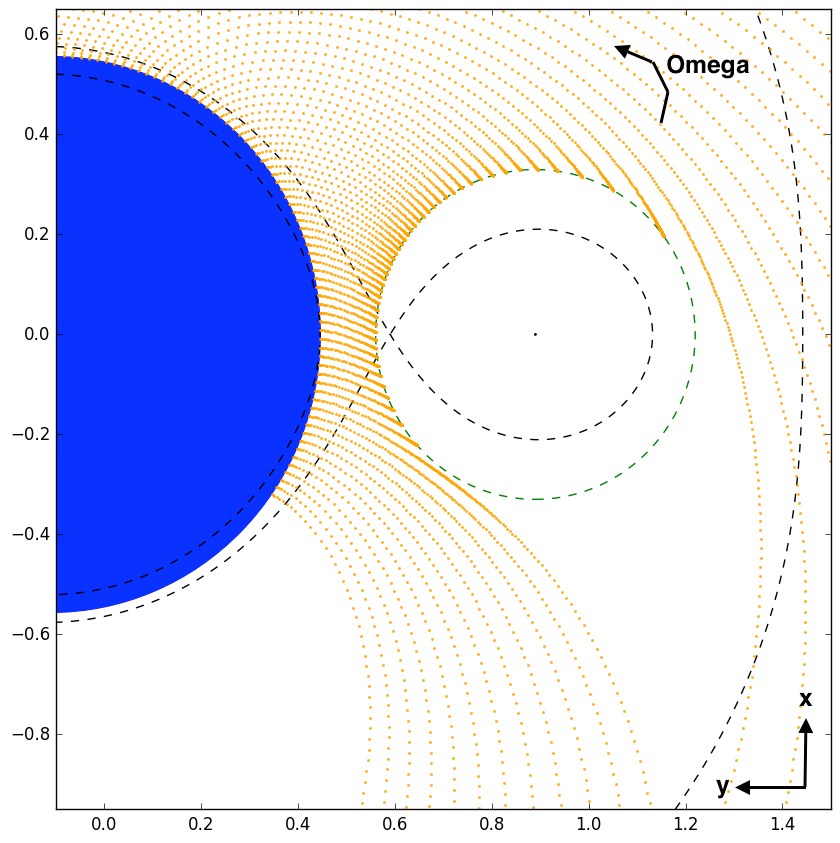
\includegraphics[width=0.9\columnwidth]{Pictures/big_picture.png}
%\caption{A few computed streamlines (orange solid lines) from the blue supergiant to the Roche lobe of the accretor on the right (green dashed circle), in the orbital plane. The black dashed lines represent the critical Roche surface passing by the first Lagrangian point. Upper panel (resp. lower) is for the heavy slow (resp. light fast) configuration.}
%\label{fig:big_picture}
%\end{figure} 

\begin{figure}
\begin{subfigure}{.5\textwidth}
\centering
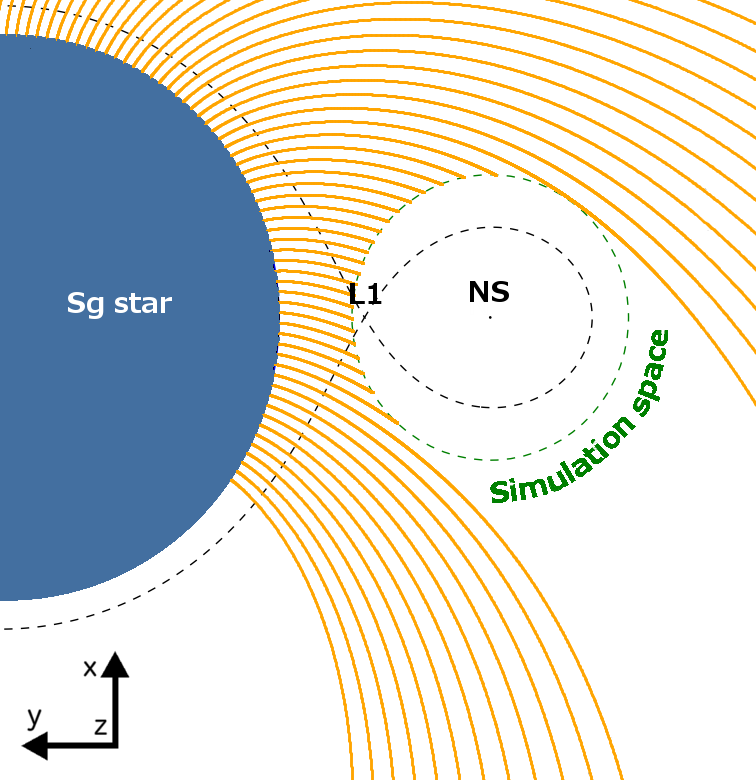
\includegraphics[width=0.99\columnwidth]{Pictures/LF.png}
  \label{fig:sfig1}
\end{subfigure}
\phantom{p}\\
\begin{subfigure}{.5\textwidth}
\centering
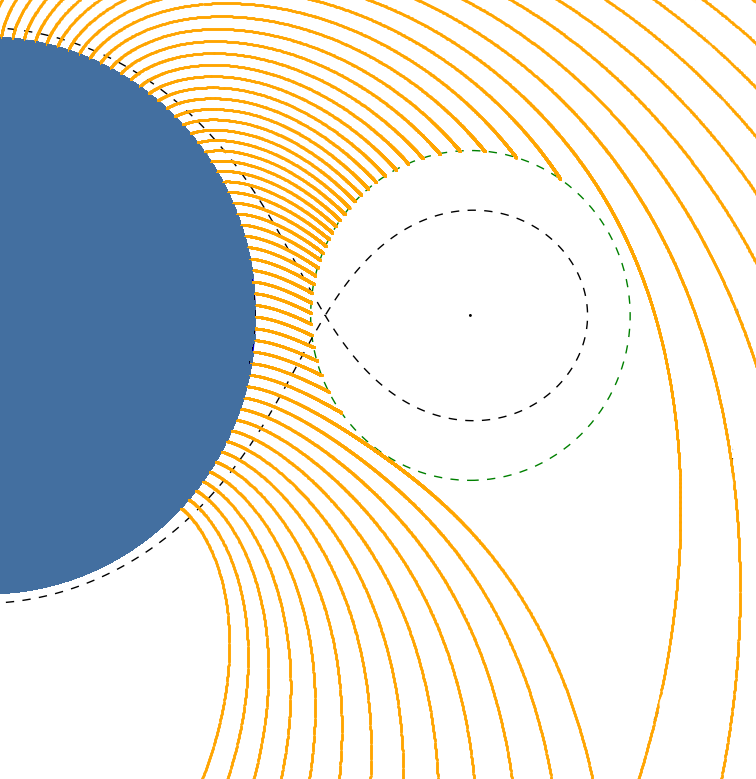
\includegraphics[width=0.99\columnwidth]{Pictures/HS.png}
  \label{fig:sfig2}
\end{subfigure}
\caption{In the orbital plane, a few computed streamlines (orange solid lines) from the blue supergiant to the hydrodynamic simulation space (green dashed circle), centered on the accreting NS. The black dashed lines represent the critical Roche surface passing by the first Lagrangian point (L$_1$). Upper panel (resp. lower) is for the light fast (resp. heavy slow) configuration.}
\label{fig:big_picture}
\end{figure} 

\begin{center}
\begin{table}
\caption{Parameters and integrated quantities at the outer edge of the simulation space for the 2 models considered.}
\label{tab:params}
\centering
\begin{tabularx}{0.53\columnwidth}{c|c|c}
   & LF & HS \\
  \hline
  M$_{\text{\mystar}}$ & \multicolumn{2}{c}{20.2M$_{\odot}$} \\
  R$_{\text{\mystar}}$ & \multicolumn{2}{c}{28.4R$_{\odot}$} \\
  P$=2\pi/\Omega$ & \multicolumn{2}{c}{8.964357 days} \\  
  a$/$R$_{\text{\mystar}}$ & \multicolumn{2}{c}{$\sim$1.8}\\
  $\dot{\text{M}}_{\text{\mystar}}$ & \multicolumn{2}{c}{6.3$\cdot$10$^{-7}$M$_{\odot}\cdot$yr$^{-1}$} \\
  \hline
  M$_{\bullet}$ & 1.5M$_{\odot}$  & 2.5M$_{\odot}$  \\
  Boosted & Yes & No  \\
  \hline
  $\dot{\text{M}}_{\text{out}}/\dot{\text{M}}_{\text{\mystar}}$ & 4\% & 17\% \\
  $l_{\text{out}}/a^2\Omega$ & -1\% & 3\% \\
  R$_{\text{circ}}$ / R$_{\text{mag}}$ & 4 & 30 \\
\end{tabularx}
\end{table}
\end{center}

Sophisticated models and simulations of the launching of line-driven winds show that they become supersonic shortly above the stellar photosphere. It motivates a ballistic treatment of the wind bulk motion at the orbital scale similar to what was done in \cite{ElMellah2016} : the trajectory of test-masses is integrated assuming the star and the accretor are on circular orbits and that stellar rotation is synchronized with the orbital period. The 3D equation of motion in the co-rotating frame is :
\begin{equation}
\label{eq:ball}
\boldsymbol{v}\frac{\diff \boldsymbol{v}}{\diff \boldsymbol{r}} = \boldsymbol{a}_{\text{\mystar}} + \boldsymbol{a}_{\bullet} + \boldsymbol{a}_{\text{ni}}
\end{equation}
where $\boldsymbol{a}_{\bullet}$ stands for the acceleration due to the \ns gravitational field and $\boldsymbol{a}_{\text{ni}}$ for the non-inertial acceleration (centrifugal and Coriolis). The effective acceleration linked to the donor star of mass $M_1$, once projected on the radial unity vector of the spherical frame of the star, is given by :
\begin{equation}
a_{\text{\mystar}}=-\frac{GM_1}{r_1^2}+a_{\text{rad}}\left(r_1\right)+a_{\text{press}}\left(r_1\right)
\end{equation}
where $a_{\text{press}}$ is the acceleration due to thermal and turbulent pressure, important near the stellar photosphere. For describing the total radiative acceleration $a_{\text{rad}}$, containing both the line and total continuum contribution, we rely on the computation by \cite{Sander2017} for Vela X-1. Using the stellar atmosphere code PoWR \citep[e.g.]{Hamann1998,Grafener2002}, they calculate an atmosphere model for the donor star assuming a spherical, stationary wind situation. The radiative transfer is performed in the comoving frame, allowing to obtain the radiative acceleration without any further assumptions or parameterizations, i.e. :
\begin{equation}
\label{eq:araddef}
a_{\text{rad}}\left(r_1\right)  = \frac{4\pi}{c} \frac{1}{\rho(r_1)}  \int\limits_{0}^{\infty} \kappa_\nu H_\nu \mathrm{d}\nu 
\end{equation}
where the mass density $\rho$ is deduced from the mass loss rate and the velocity using the conservation of mass. Using the technique described in \cite{Sander2017b}, the model provides a hydrodynamically consistent stratification, meaning that the mass-loss rate and the velocity field were iteratively updated such that eventually the outward and inward forces are balancing each other throughout the stellar atmosphere. The resulting velocity and density stratification shows notable deviations from the typically assumed $\beta$-law, especially within a couple of stellar radii, where the orbiting accretor lies and where the obtained wind velocity is lower. Notice that in spite of the non-spherical situation due to the presence of the \ns, we adopt $a_\text{rad}$ as $a_\text{press}$ as functions of the distance $r_1$ to the donor star here for simplicity.

The streamlines computation is performed using the code developed in \cite{ElMellah2016a}, starting from the stellar surface whose ellipsoidal deformation, even for Roche lobe filling factors close to unity, is expected to have a negligible impact on the formation of a wind-capture disc. An illustration of the result is given in Figure\,\ref{fig:big_picture} where the streamlines have been represented in the orbital plane. We stop the integration when the test-masses enter a sphere around the accretor $\sim$30\% larger than its Roche lobe radius. This strategy alleviates the difficulty of an a priori estimate of the accretion radius \citep[the critical impact parameter below which test-masses are captured in the Bondi-Hoyle-Lyttleton formalism][]{Edgar:2004ip}. It delimits the space where the ballistic approximation no longer holds. Dissipative effects will be accounted for within this region in section\,\ref{sec:wind-capt_discs}. With this procedure, we focus on the fraction of the flow susceptible to be eventually accreted rather than on an accurate representation of the accretion tail in the wake of the accretor \citep[for this component, see rather][]{Manousakis2013}.

\cite{Vink2001} showed that, provided the stellar effective temperature is larger than $\sim$25kK, the wind terminal speed is expected to scale approximately as the effective escape velocity (\ie once surface gravity has been corrected for radiative continuum pressure on free electrons via the Eddington parameter). Below this critical temperature, the terminal speed with respect to the effective escape speed of the star drops steeply. The donor star in Vela X-1, HD77581, is a B0.5 Ib supergiant star \citep{Hiltner1972,Forman1973} whose effective temperature of $\sim$25kK. \cite{Gimenez-Garcia2016} suggested that it could explain the low terminal speed of 700km$\cdot$s$^{-1}\pm$100km$\cdot$s$^{-1}$ they measured for the wind of HD77581. The computation carried on by \cite{Sanders2017} for HD77581 also leads to terminal speeds ranging from 400 to 600km$\cdot$s$^{-1}$ depending on the inclusion of X-ray illumination from the accretor. A decisive result of their analysis is that the latter modifies the ionization state of the metal ions in the wind but does not necessarily inhibit the acceleration process. On the contrary, far enough upstream the \ns, the effective absorption of UV photons might be locally enhanced once the metal ions are in a higher ionization level. It is only close from the accretor, once all the elements have been deprived of their electrons, that the line-driven acceleration is halted, as previously emphasized in the literature \citep[see \eg][]{Blondin1990a}. XXX ANDREAS : DO YOU CONFIRM? WOULD YOU REFORMULATE? SHOULD IT BE AN ENTIRE SUBSECTION TO CLEARLY MAKE THIS POINT? XXX In an attempt to illustrate the dramatic impact of the efficiency of the line-driven acceleration on the subsequent properties of the accretion flow, and to encompass potential biases in the calculation of this acceleration, we consider the case of an artificially enhanced wind acceleration (by 50\%) which leads to larger flow velocities by approximately 20\%. In section\,\ref{sec:wind-capt_discs}, we will see that the orbital speed is a threshold which separates two types of accretion flows and given the value of the orbital speed in Vela X-1 (284km$\cdot$s$^{-1}$), this wind acceleration boosting will induce major changes. From now on, we consider the two cases in Table\,\ref{tab:params} :
\begin{itemize}
\item \underline{the heavy slow (HS) :} the accretor has a mass of M$_{\bullet}$=2.5\msun, lying on the upper edge of the expected maximum mass for a \ns, and the radiative acceleration is not boosted.
\item  \underline{the light fast (LF) :} the accretor has a mass of M$_{\bullet}$=1.5\msun and the radiative acceleration is boosted by 50\%.
\end{itemize} 
Since the \ns mass estimates in Vela X-1 range from 1.7\msun \citep{Rawls2011} up to 2.3\msun \citep{Quaintrell2003a}, partly due to the uncertainty on the inclination of the system, we expect the real configuration to lie in-between the two cases we consider.

% - - - - - - - - - - - - - - - - - - - - - - - - 
\subsection{Inhomogeneity and asymmetry of the wind}
\label{sec:orb_inhomo}
% - - - - - - - - - - - - - - - - - - - - - - - - 

\begin{figure*}
\centering
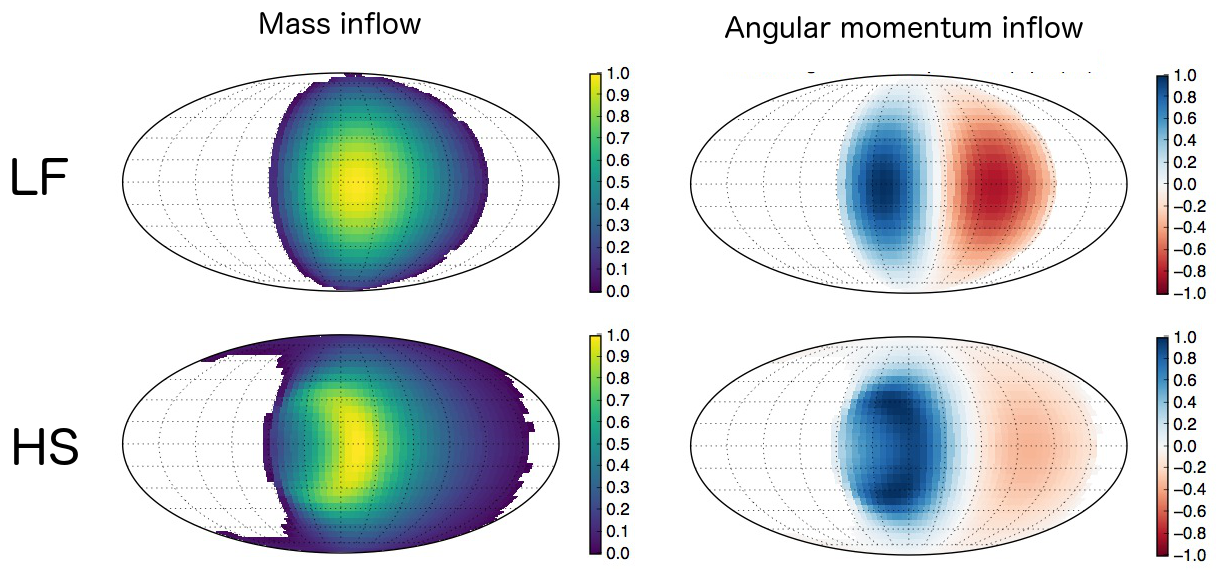
\includegraphics[width=2\columnwidth]{Pictures/inflow_maps.png}
\caption{Mollweide projections of local mass and angular momentum inflows within the simulation space centered on the accretor (dashed green sphere on Figure\ref{fig:big_picture}). The upper row corresponds to the light fast (LF) case while the bottom row is for the heavy slow (HS) case. Each map is scaled to its maximum (absolute) value and centered on the axis from the accretor to the donor star. Positive (resp. negative) values of angular momentum stands for locally prograde (resp. retrograde) flow with respect to the orbital motion. The color maps have been scaled using the maximum (absolute) value in each plot.}
\label{fig:inflow_maps}
\end{figure*} 

We now monitor the flow as it enters the spherical HD simulation space centered on the compact object and corresponding approximately to its Roche lobe. The aforementioned ballistic integration supplied information on the velocity vector at the surface of this sphere while the density relative to the stellar one is deduced from the divergence of each streamline. This information is then binned on angular tiles, with the polar axis of the spherical frame aligned with the orbital angular momentum axis ($\hat{z}$ in Figure\,\ref{fig:big_picture}). We represented the local mass and angular momentum inflow at the surface of this space with Mollweide projection in Figure\,\ref{fig:inflow_maps} for the HS and LF cases : it offers an overview of the properties of the flow entering the accretor Roche lobe, as seen from the accretor. 

Concerning the integrated values at the outer inflowing edge of the simulation space, we focus on the mass inflow rate, the net specific (\ie per unit mass) angular momentum of the flow and its corresponding circularization radius. The latter is the radius at which a Keplerian orbit would have the same specific angular momentum. The values are given in Table\,\ref{tab:params} and compared respectively to the stellar mass loss rate, to the orbital specific angular momentum and to the \ns magnetosphere radius, given by \citep{Martinez-Nunez2017} :

%Their integrated value, $\dot{\text{M}}_{\text{out}}$ and $\dot{\text{j}}_{\text{out}}$, normalized with the corresponding scaling parameters. Dividing the accretion rates of angular momentum and mass, we obtain the specific angular momentum of the inflowing gas and can compute the radius at which a Keplerian orbit would have the same specific angular momentum (\aka the circularization radius). 

%This radius is compared to the \ns magnetosphere radius, $R_{\text{mag}}$, given by \cite{Martinez-Nunez2017} :

\begin{align}
\begin{split}
\label{eq:Rmag}
R_{\text{mag}}\sim & 1.4\cdot 10^9\text{cm}\left(\frac{\rho}{10^{-12}\text{g}\cdot\text{cm}^{-3}}\right)^{-1/6}\left(\frac{v}{2,000\text{km}\cdot\text{s}^{-1}}\right)^{-1/3} \text{...}\\
& \text{...} \quad \left(\frac{B_{\bullet}}{2.6\cdot 10^{12}\text{G}}\right)^{1/3}\left(\frac{R_{\bullet}}{10\text{km}}\right)
\end{split}
\end{align}
where the values used for the mass density $\rho$ and the flow speed $v$ are orders-of-magnitude at the outer edge of the magnetosphere. The low dependence of the magnetosphere radius on them guarantees that their exact value will not significantly alter this estimate. A typical \ns radius has been used and the \ns magnetic field is the one deduced by \cite{Furst2014} in Vela X-1. In Table\,\ref{tab:params}, we used R$_{\text{mag}}=$1.4$\cdot$10$^9$cm. We expect any disc-like structure to be truncated approximately at the inner radius \citep{Ghosh1978} while quasi-spherical accretion onto the magnetosphere would proceed as described by \cite{Shakura2013b}. Notice that the mass inflow rate sets only an upper limit on the final rate at which matter will be accreted, while the angular momentum might still vary within the simulation space : the results displayed in Table\,\ref{tab:params} serve to show that, within the current uncertainties on the mass of the accretor and on the efficiency of the wind launching process in Vela X-1, the 2 cases lead to dramatically different accretion flow configurations, in spite of their apparently similar parameters. In the HS case, where the flow is slightly slower than the orbital speed, the mass inflow rate within the Roche lobe of the accretor is 4 times larger, while the circularization radius is almost an order of magnitude larger than in the LF case, where the flow is slightly faster than the orbital speed. 

On the left panels in Figure\,\ref{fig:inflow_maps}, we see that the mass inflow is approximately distributed in the same way in both cases, with a larger off-plane contribution when the wind is slower : it is a first hint that the inertia of the wind is no longer large enough to overcome the orbital beaming induced by rotation, a feature which will have major consequences within the shocked region. In both cases, the incoming flow is centered around a mean direction which departs from the axis joining the compact object to the star. The essential difference though lies in the distribution of angular momentum inflow (right panels) : the LF case leads to an equivalent amount of positive and negative angular momentum, revealing of the essentially planar (albeit deviated) structure of the flow, whereas the HS case displays a large unbalance. The evaluation of the net angular momentum inflowing was in no case obvious a priori : the flow arriving from the first Lagrangian point L$_1$ (with positive angular momentum) is denser than the flow arriving from the right of L$_1$ as seen from the accretor (with negative angular momentum), but it is also slower. The present analysis was required to determine which effect eventually dominates. The non-zero net angular momentum in the HS case can not be attributed to an asymmetry of the mass inflow. Rather, it is due to the shift between the mean direction of arrival of matter (yellow spot in mass inflow maps) and the direction of radial inflow (white stripe in-between blue and red in angular momentum inflow maps). It is much more significant for HS than for LF. Consequently, the net amount of specific angular momentum is larger for HS, which also leads to larger circularization radii and to a likelier wind-capture disc, a prediction we now put to the test.

% ------------------------------------------------
\section{Wind-capture discs}
\label{sec:wind-capt_discs}
% ------------------------------------------------

% - - - - - - - - - - - - - - - - - - - - - - - - 
\subsection{Physics and numerical setup}
\label{sec:HD}
% - - - - - - - - - - - - - - - - - - - - - - - - 

\subsubsection{Equations}
\label{sec:HD_eq}
%normalization units?

Within the Roche lobe of the accretor, we solve the equations of hydrodynamics in their conservative form, converting accordingly the gravitational, radiative and non-inertial accelerations in the ballistic equation of motion\,\eqref{eq:ball} into forces per unit volume. In a first time, we do solve the energy equation everywhere, assuming that the heating from the donor star and from the X-ray produced in the vicinity of the accretor balances the cooling of this radiatively thin supersonic wind. We will discuss the validity of this adiabatic approximation downstream the shock which will form and a way to relax it in section\,\ref{sec:cool}. Finally, we complement these equation with the equation-of-state of an ideal monoatomic gas of Hydrogen (\ie with an adiabatic index $\gamma=5/3$) as a closure relation, which gives the internal energy per unit volume $u$ as a function of the thermal pressure $P$. We also set the mean molecular weight to unity, to be used in the estimates of the cooling time scale in section\,\ref{sec:cool}.

The computation is performed with the new version of the finite volume code \texttt{MPI-AMRVAC} \citep{Xia2017}, using a 3$^{\text{rd}}$ order HLL solver \citep{Toro1994} with a Koren slope limiter \citep{Vreugdenhil1993}. The spherical mesh we set up, centered on the accretor, is radially stretched to guarantee a constant relative resolution from the outer to the inner edge of the simulation space, spanning several orders of magnitude at an affordable computational cost and with a uniform cell aspect ratio, extending what has been done for an axisymmetric 2D flow in \cite{ElMellah2015}. The outer radius of the simulation space is approximately half of the orbital separation, which is $\sim$0.2AU in Vela X-1, while the inner edge has a radius of 5 times the \ns magnetosphere radius given by equation\,\eqref{eq:Rmag}, hence a factor of approximately 200 between the inner and outer edge. Due to the symmetry of the problem above and below the orbital plane, we consider only the upper hemisphere and work with a resolution of 128$\times$32$\times$128 corresponding to cells of aspect ratio close to unity near the equatorial plane of the mesh. Since our aim is to identify the conditions suitable for the formation of a wind-capture disc, the conservation of angular momentum is of uttermost importance. We implemented an angular momentum preserving scheme which guarantees the conservation of the component of the angular momentum projected onto the polar axis, in particular in the innermost regions of the flow, to machine precision (XXX RONY : WOULD YOU HAVE A REFERENCE IN MIND? XXX). However, we confirm that our results remained essentially unchanged by setting the polar axis in the orbital plane (but still orthogonal to the line joining the star to the compact object), which empirically verifies that \texttt{MPI-AMRVAC} properly handles the polar singularity.

%\begin{equation}
%\label{eq:eq1}
%%\tag{1a}
%\partial _t \rho + \boldsymbol{\nabla} \cdot \left( \rho \boldsymbol{v} \right) = 0
%\end{equation}
%\begin{equation}
%\label{eq:eq2}
%%\tag{1b}
%\partial _t \left( \rho \boldsymbol{v} \right) + \boldsymbol {\nabla} \cdot \left( \rho \boldsymbol{v} \boldsymbol{v} + P \mathbb{1} \right) = \rho \boldsymbol{f} - 2 \boldsymbol{\Omega} \wedge \boldsymbol{v}
%\end{equation}
%\begin{equation}
%\label{eq:eq3}
%%\tag{1c}
%\partial _t  e  + \boldsymbol{\nabla} \cdot \left[ \left( e + P \right) \boldsymbol{v} \right] = - \rho \boldsymbol{v} \cdot \boldsymbol{f}
%\end{equation}
%where $\rho$, $\boldsymbol{v}$, $P$ and $e$ are the mass density, velocity, pressure and total energy density respectively. $\boldsymbol{\Omega}$ is the orbital angular speed vector. $f$ is the modified Roche force per mass unit given by : 
%
%\begin{equation}
%\boldsymbol{f}=\alpha\left( r_1 \right) \frac{q}{r_1^3}\boldsymbol{r_1} - \frac{1}{r_2^3}\boldsymbol{r_2} + \frac{1+q}{a^3}\boldsymbol{r_{\perp}}
%\end{equation}
%
%with the mass ratio $q=M_1/M_2$
%$\boldsymbol{r_1}$
%$\boldsymbol{r_2}$
%$\boldsymbol{r_{\perp}}$
%$\alpha$ : see section\,\ref{sec:wind_acc}. Encapsulates wind acceleration process and stellar gravity. $-1$ with only gravity, leading to the usual Roche force per unit mass.


\subsubsection{Radiative cooling}
\label{sec:cool}

Let us estimate the importance of cooling in these simulations. Upstream the shock, we rely on the temperature stratification derived from the solution of the statistical equilibrium equations and the radiative transfer. Based on the assumption of radiative equilibrium, the (electron) temperature structure in an expanding atmosphere is obtained by applying a generalized Uns{\"o}ld-Lucy method described in \citet{Hamann1998}. Including the X-ray irradiation on the donor star did not significantly alter the temperature profile upstream the accretor obtained in \cite{Sander2017}, leading to wind temperatures of 15 to 20kK. XXX ANDREAS : DO YOU CONFIRM THE CONTENT AND THE FORM? XXX. Downstream the shock, we assume that the gas is still optically thin and consider the time scale $\tau_{\text{c}}$ to evacuate the internal energy per unit volume of an ideal gas at temperature $T$ and with a Hydrogen number density $n$, $u=nk_{\text{B}}T$, at a rate given by the cooling rate computed by \cite{Schure2009}, $\Lambda\left(T\right)$ :
\begin{equation}
\tau_{\text{c}}=\frac{nk_{\text{B}}T}{n^2\Lambda\left(T\right)}
\end{equation}
where $\Lambda$ includes the proportion of electrons relative to protons and $k_{\text{B}}$ is the Boltzmann constant. If we write $\tau_{\text{d}}$ the dynamical time scale for free fall at a fiducial accretion radius R$_{\text{acc}}$ of 1$/$30$^{\text{th}}$ of the orbital separation in Vela X-1, we obtain the following ratio :
\begin{align}
\frac{\tau_{\text{c}}}{\tau_{\text{d}}}\sim & 0.01\left(\frac{T}{10^6\text{K}}\right)\left(\frac{\Lambda}{10^{-22}\text{erg}\cdot\text{s}^{-1}\cdot\text{cm}^{3}}\right)^{-1} \text{...}\\
&  \text{...} \quad \left(\frac{\rho}{10^{-13}\text{g}\cdot\text{cm}^{-3}}\right)^{-1}\left(\frac{M_{\bullet}}{2\text{M}_{\odot}}\right)^{1/2}\left(\frac{\text{R}_{\text{acc}}}{0.2\text{AU}/30}\right)^{-3/2}
\end{align}
where we used the values of temperature and density measured downstream the shock in the adiabatic simulations presented in section\,\ref{sec:cool_F}. It is clear that, except if the wind is a few times faster than expected in Vela X-1 and/or the star displays a mass loss rate an order of magnitude lower than what models and observations indicate \cite[$\sim$1.3$\cdot 10^{-6}$M$_{\odot}\cdot$yr$^{-1}$,][]{Gimenez-Garcia2016}, cooling will come into play in the shocked region. 

In an optically thin environment, we could include radiative cooling using the module developed for \texttt{MPI-AMRVAC} by \cite{VanMarle2011}. However, we would also need to model heating by X-rays from the compact object and by the stellar radiation field, and to use power-law approximations to compute the local opacity as a function of the density and the temperature \citep{Lin1985}. Furthermore, the optically thin approximation might not hold within the shocked region, especially when runaway cooling occurs and a high density disc-like region forms. In optically thick region, the strong coupling between matter and radiation requires more sophisticated treatments such as flux-limited diffusion \citep{Turner2001}. XXX RONY : SHOULD WE CITE JANNIS' PAPER HERE? XXX Given the additional layers of complexity a proper treatment of radiation would add, we chose to represent the cooling in a simpler way, using a polytropic model. It is equivalent to assume that the ratio of energy radiated away by the work of done by pressure force is constant : a certain compression leads to a certain energy loss, ranging from 0 (in the adiabatic limit) to 100\% (in the isothermal limit) of the work done by pressure force \citep{Christians2012}. Above a certain threshold temperature T$_{0}$, reached only within the shocked region, we overwrite the solution for the internal energy computed by the energy equation with the corresponding value of pressure deduced from the polytropic relation :
\begin{equation}
P=C\rho^{\alpha}
\end{equation}
Provided there is no creation of entropy (in particular no shock), $C$ is constant and uniform. In this framework, the polytropic index $\alpha$ ranges from 1 in the isothermal limit to $\gamma$ in the adiabatic limit \citep{Horedt2000}. After exploring a range of realistic values for $C$ and $\alpha$, we retained 3 different models :
\begin{itemize}
\item \underline{High entropy :} cooling occurs only in a thin unresolved radiative layer immediately downstream the shock and is then negligible (for instance, because of intense X-ray heating) which means $\alpha=\gamma$ and a constant $C$ set to a fraction of the entropy the flow would acquire downstream the shock in the fully adiabatic case, $S_0$. T$_{0}$ is set to 10$^6$K.
\item \underline{Isothermal hot :} the net cooling is efficient enough to compensate any adiabatic compression as the flow accretes, which leads to an isothermal flow ($\alpha=1$) whose temperature is given by $C$, set such as the physical temperature is 10$^6$K. 
\item \underline{Isothermal cool :} same as previous but with a temperature of 10$^5$K.
\end{itemize}
In the two isothermal cases, the cooling prescription means that the flow evolution is fully adiabatic until it reaches the temperature $T_0=C$ when it becomes isothermal. We believe that including the optically thin cooling without heating would lead to results qualitatively similar to the isothermal prescription we introduce here \citep[as noticed by][]{Saladino2018} . The four models (fully adiabatic, high entropy, isothermal hot and cold) are summarized in Table\,\ref{tab:cool}.

\begin{table}
\centering
\caption{Parameters of cooling prescriptions in the four models.}
\label{tab:cool}
\begin{tabularx}{0.78\columnwidth}{c|c|c|c|c}
   & adiabatic & isoS & Hot & Cool\\
  \hline
  Cooling & no & yes & yes & yes \\  
  $T_0$ & -- & 10$^6$K & 10$^6$K & 10$^5$K \\
  $C$ & -- & $S_0$ & $T_0$ & $T_0$ \\
  $\alpha$ & -- & $\gamma$ & 1 & 1 \\
\end{tabularx}
\end{table}

% - - - - - - - - - - - - - - - - - - - - - - - - 
\subsection{Flow morphology}
\label{sec:morph}
% - - - - - - - - - - - - - - - - - - - - - - - - 

\subsubsection{Adiabatic evolution}
\label{sec:cool_F}

\begin{figure}
\begin{subfigure}{.5\textwidth}
\centering
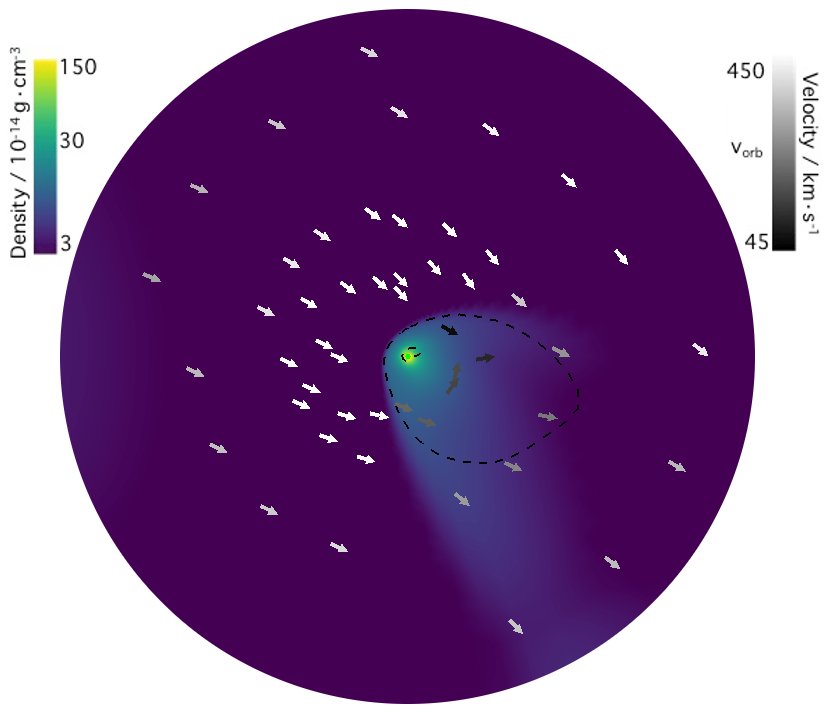
\includegraphics[width=0.99\columnwidth]{Pictures/LF_adiab.jpeg}
  \label{fig:sfig1}
\end{subfigure}
\begin{subfigure}{.5\textwidth}
\centering
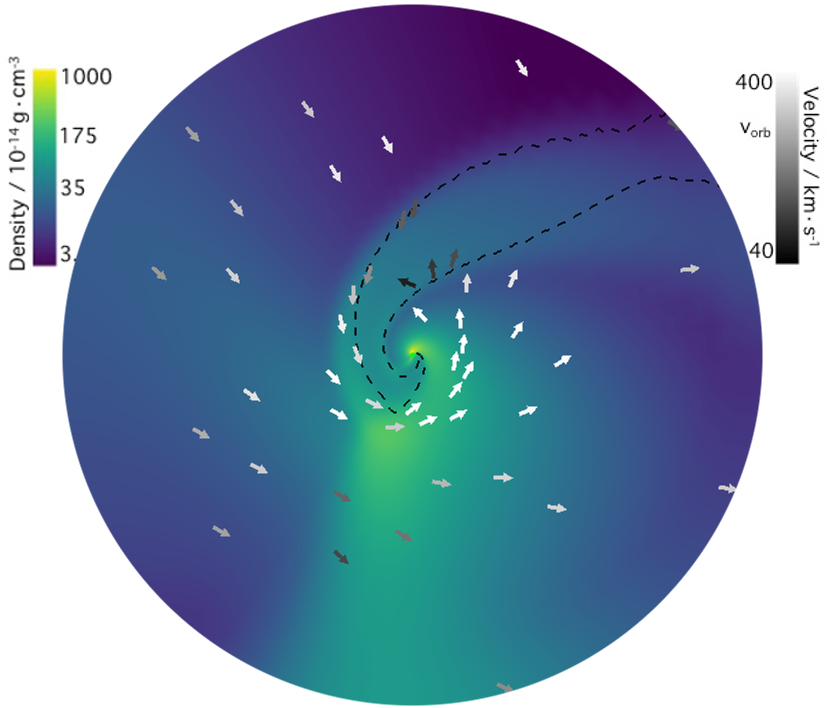
\includegraphics[width=0.99\columnwidth]{Pictures/HS_adiab.jpeg}
  \label{fig:sfig2}
\end{subfigure}
\caption{Logarithmic colormaps of the density field in the orbital plane. The arrows stand for the velocity field, with a black to white colormap for their magnitude. The black dashed line is the Mach-1 contour. The orbital speed of Vela X-1, v$_{\text{orb}}\sim284$km$\cdot$s$^{-1}$ has been represented. The radial extension of the simulation domains relative to the orbital separation is given by the green dashed delimited region in Figure\,\ref{fig:big_picture}.}
\label{fig:adiab}
\end{figure} 

In Figure\,\ref{fig:adiab}, we represented slices in the orbital plane of the numerically relaxed state reached by the simulations where the adiabatic equations of hydrodynamics are solved. A 3D representation is displayed in Figure\,\ref{fig:3D_adiab} to appreciate the level of beaming of the flow along the orbital axis.

In the case of a light accretor capturing material from a fast wind (LF configuration), the main features depart little from what has been observed for axisymmetric uniform flows. In agreement with \cite{Blondin:2012vf}, we do not observe any transverse oscillation of the tail \citep[the so-called "flip-flop instability" which arises in 2D polar numerical setups,][]{Foglizzo2005}. The orbital effects deflected the wind whose mean direction of arrival is $\sim$20 degrees misaligned with respect to the axis joining the star to the compact object. However, as discussed in section\,\ref{sec:orb_inhomo}, the flow remains essentially planar around this direction. When the flow is sufficiently beamed towards the accretor, it forms a bow shock at a distance ahead the accretor compatible with a fraction of the previously estimated accretion radius. The Mach-1 surface and the cone of density jump are slightly misaligned with each other, with the side facing the star denser. The Mach number immediately upstream the shock reaches 30 and we retrieve the classic jump conditions for an adiabatic shock. Between the outer boundary upstream and the inner boundary, the density (resp. the temperature) increases by a factor of $\sim$100 (resp. 5,000). In the innermost regions of the flow, we retrieve the sonic surface though no longer anchored into the inner boundary, contrary to what was predicted for a planar uniform flow with $\gamma=5/3$ by \cite{Foglizzo1996} and observed by \cite{ElMellah2015} in numerical simulations.

In the case of a heavy accretor capturing material from a slow wind (HS configuration), the morphology of the flow is dramatically different. Not only is the mean direction of arrival of the flow more misaligned with the line joining the star to the compact object ($\sim$45 degrees) but also the shearing is much more important, leading to a significant amount of net angular momentum. A bow shock also forms but while it extends over several accretion radii on the side where the flow is less dense and faster, the beamed wind arriving directly from L$_1$ remains mildly supersonic as it passes the accretor. It is strongly deflected and accelerated by the gravitational slingshot but only to finally impacts the shocked region from the back. The adiabatic compression it first experiences leads to a dense and fairly cool region compared to the innermost parts of the flow. We also notice that when the wind is slower, material from larger latitudes on the star contributes to the accretion process, as shown by the vertical extent of the mass inflow map in Figure\,\ref{fig:inflow_maps} : its beaming in the orbital plane builds up the red dark bulge observed on the right in Figure\,\ref{fig:3D_adiab}. Although the Mach number of the flow entering the simulation space remains below 10 due to the limited efficient of the wind acceleration, it reaches Mach numbers of 20 just upstream the shock, leading to a temperature jump of approximately 400. As the flow is accreted, the corresponding temperatures of the order of 10MK keeps increasing up to 100MK at the inner boundary. In the absence of radiative cooling, these temperatures are to be expected but as explained in section\,\ref{sec:cool}, the density of the flow is too high to neglect the capacity of the flow to radiate internal energy away. Finally, the shocked region presents a characteristic spiral shape which delimits a narrow accretion channel along which matter flows in (or out beyond the stagnation point). The orientation of this stream differs in its orientation with the one observed in \rlof systems due to the much lower effective gravity of the donor star, which alters the classic Roche potential we rely on in low mass X-ray binaries.

\begin{figure}
\centering
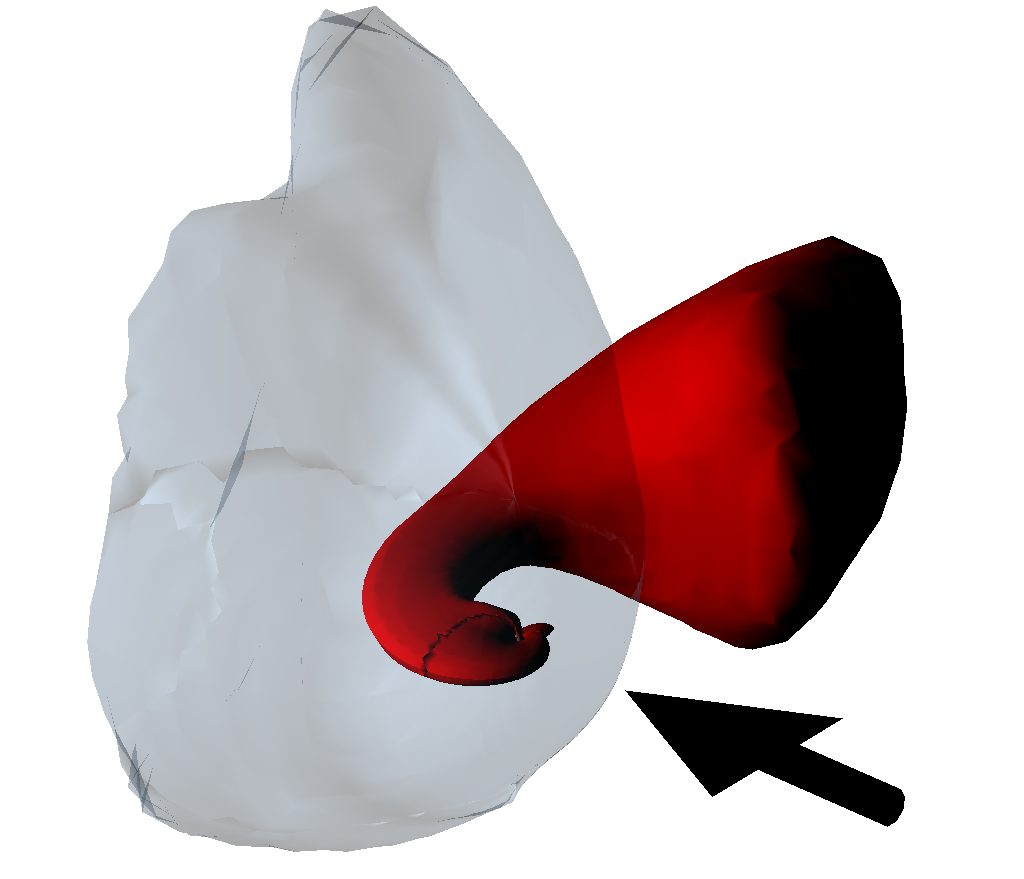
\includegraphics[width=0.99\columnwidth]{Pictures/iso-rho_adiab.png}
\caption{3D contours of the mass density for the LF (semi-transparent blue) and HS (red) configurations. The black arrow indicates the approximate direction of the arriving wind, while the vertical direction is aligned with the orbital angular momentum. Notice the axisymmetry of the LF flow structure, whereas the HS flow is compressed in the orbital plane and forms a characteristic channel reminiscent of the stream of matter in \rlof systems. Same scale as Figure\,\ref{fig:adiab}.}
\label{fig:3D_adiab}
\end{figure} 

\subsubsection{Polytropic cooling}
\label{sec:cool_T}

\begin{figure*}
\begin{subfigure}{0.5\textwidth}
\begin{center}
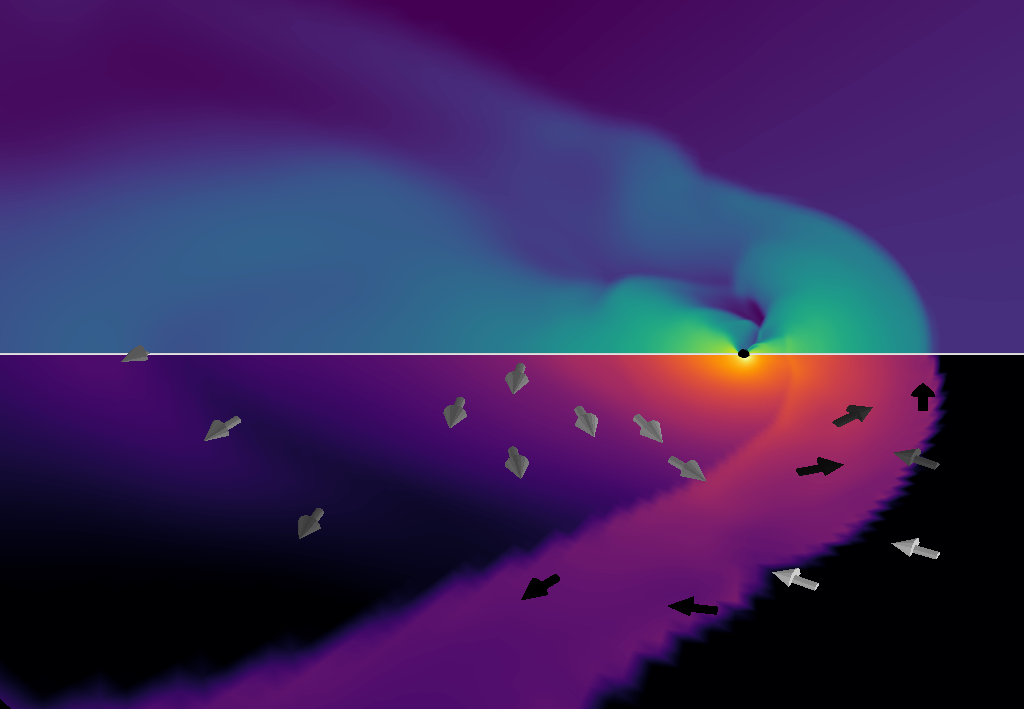
\includegraphics[width=8.6cm]{Pictures/isoS_1.png} 
\label{fig:subim1}
\end{center}
\end{subfigure}
\begin{subfigure}{0.5\textwidth}
\begin{center}
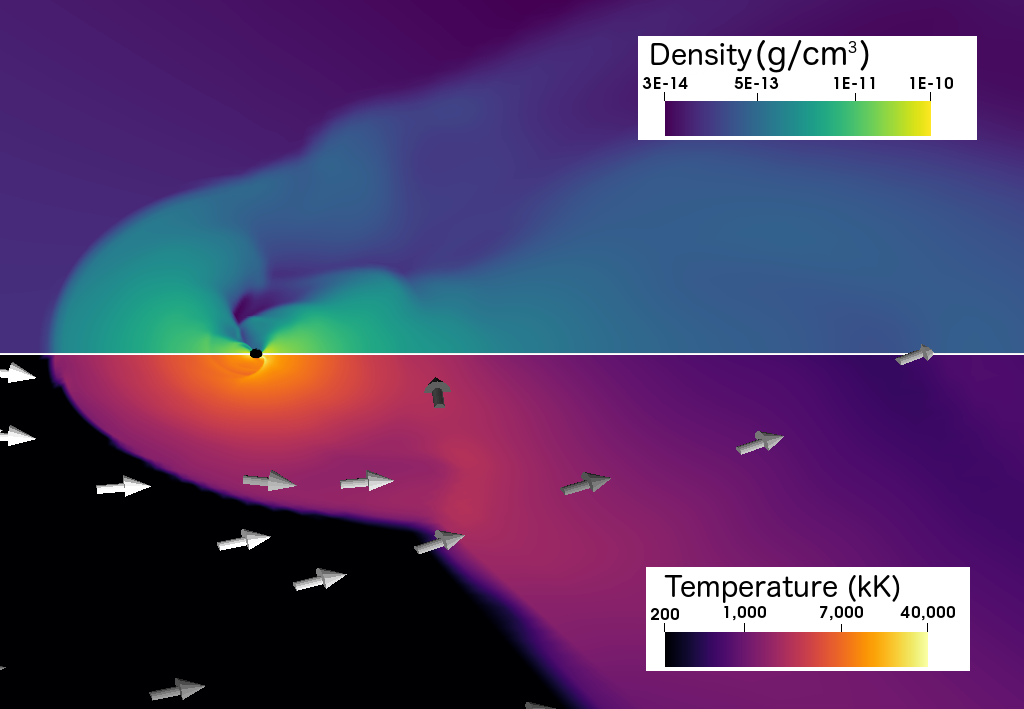
\includegraphics[width=8.6cm]{Pictures/isoS_2.png}
\label{fig:subim2}
\end{center}
\end{subfigure}
\vspace*{0.8cm}\\
\hspace*{-0.2cm}
\begin{subfigure}{0.5\textwidth}
\begin{center}
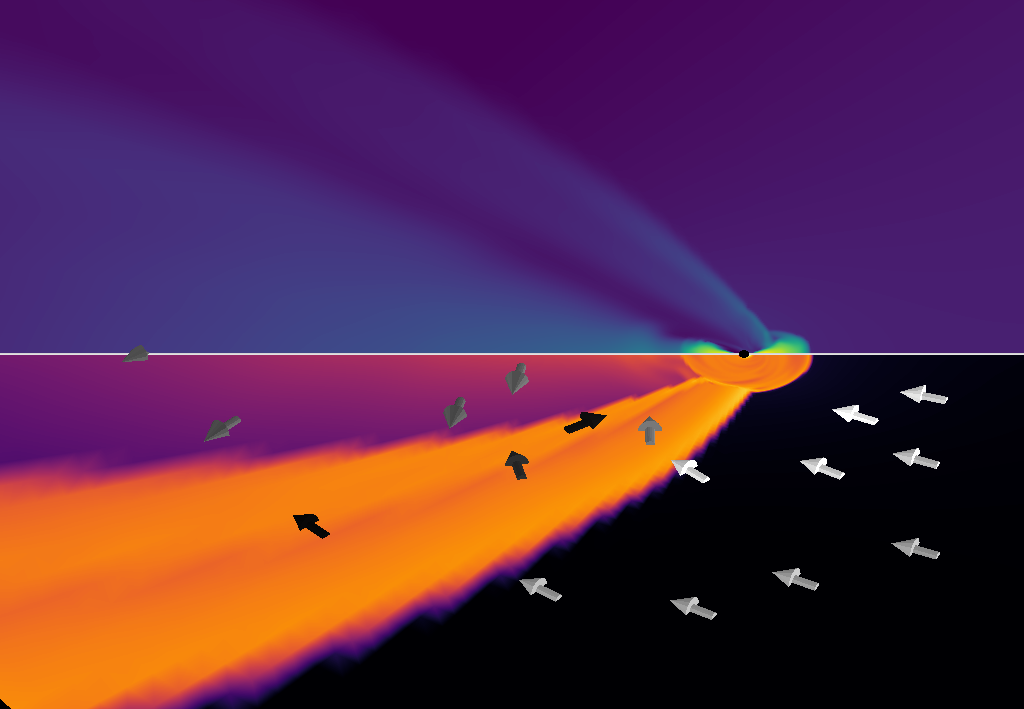
\includegraphics[width=8.6cm]{Pictures/isoHot_1.png}
\label{fig:subim2}
\end{center}
\end{subfigure}
\begin{subfigure}{0.5\textwidth}
\begin{center}
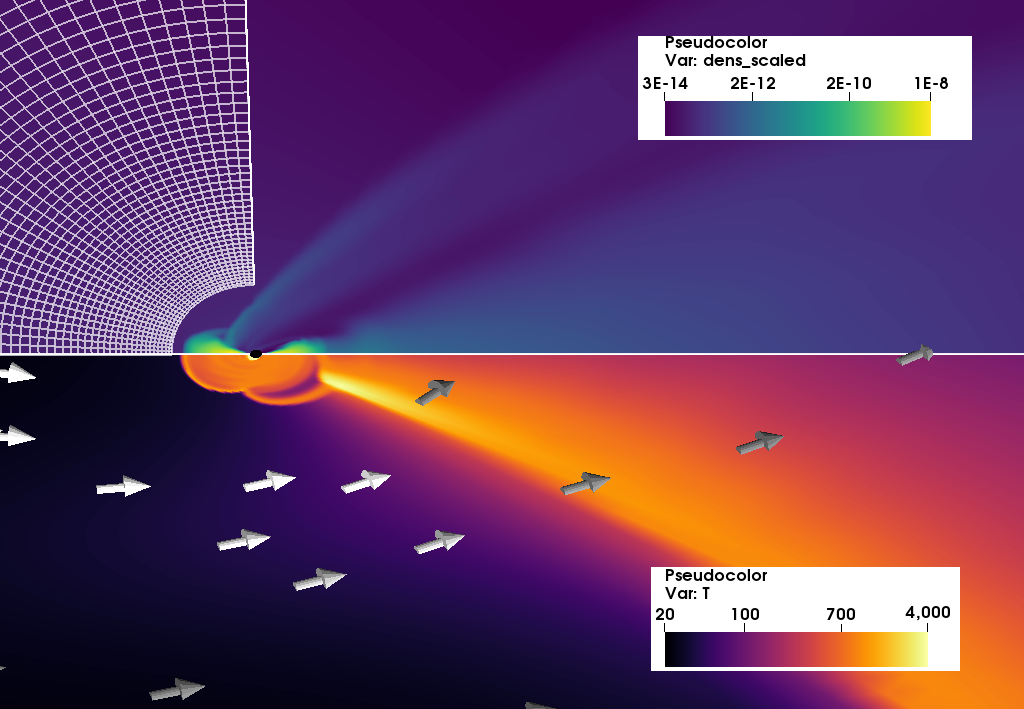
\includegraphics[width=8.6cm]{Pictures/isoHot_2.png} 
\label{fig:subim1}
\end{center}
\end{subfigure}
\vspace*{0.8cm}\\
\hspace*{-0.2cm}
\begin{subfigure}{0.5\textwidth}
\begin{center}
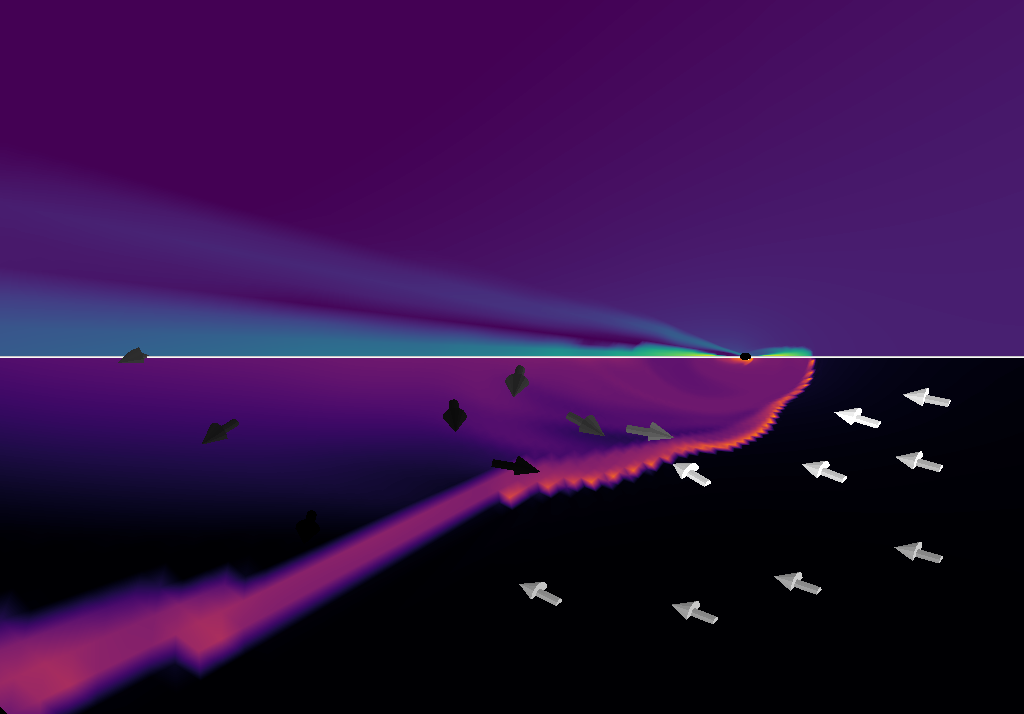
\includegraphics[width=8.6cm]{Pictures/isoCold_1.png}
\label{fig:subim2}
\end{center}
\end{subfigure}
\begin{subfigure}{0.5\textwidth}
\begin{center}
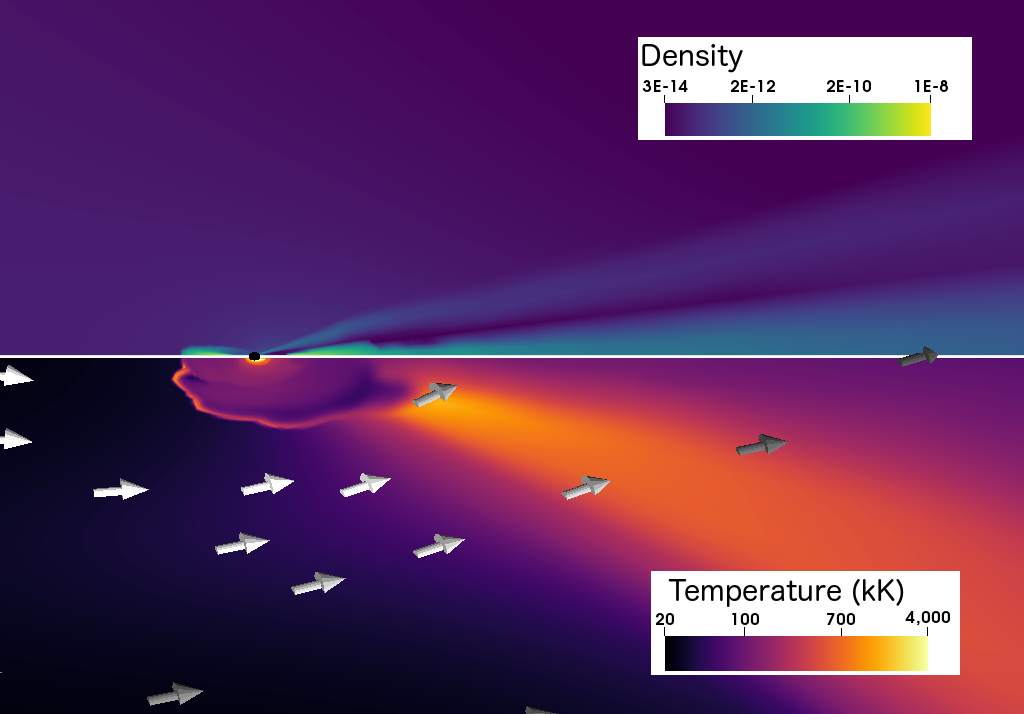
\includegraphics[width=8.6cm]{Pictures/isoCold_2.png}
\label{fig:subim2}
\end{center}
\end{subfigure}
\caption{Side-views of the flow structure when cooling is triggered using an adiabatic (upper panels) or an isothermal prescription, with a high temperature (middle) or low temperature (lower panels). The lower half of each panel displays a logarithmic thermal colormap in the orbital plane while the upper half represents the transverse logarithmic density distribution. We also plotted the velocity field in the orbital plane, with white to black color scale to indicate a slowing down by a factor of at least 4. The radially stretched mesh has been represented to indicate the resolution.}
\label{fig:cooled_ones}
\end{figure*}

\begin{figure}
\centering
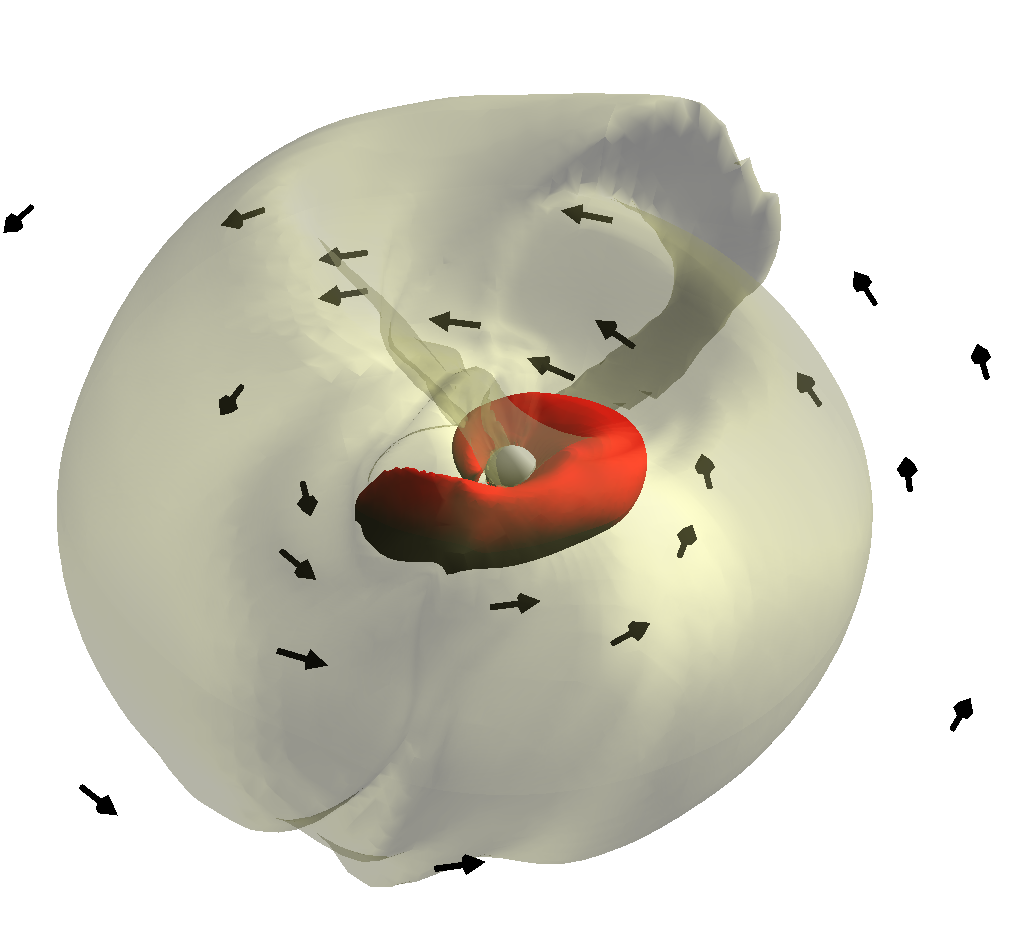
\includegraphics[width=0.99\columnwidth]{Pictures/disc.png}
\caption{3D contours of the mass density for the isentropic HS configuration (upper panels in Figure\,\ref{fig:cooled_ones}), with the yellow semi-transparent surface 5 times less dense than the inner red surface. The arrows stand for the velocity field in the orbital plane. The flow comes from the upper left. Spiral arms are visible for each surface. The central white sphere stand for the inner boundary of the simulation space, $\sim$ 200 times smaller than the outer boundary displayed in Figure\,\ref{fig:big_picture}.}
\label{fig:disc}
\end{figure} 

The case for cooling has been made in section\,\ref{sec:cool} on the base of preliminary estimates. Without cooling, we have seen that no disc formation is possible, whatever the net angular momentum carried by the accreted flow. It agrees with previous 3D numerical simulations of asymmetric Bondi-Hoyle-Lyttleton accretion, either in the context of common envelope phase \citep{MacLeod2014} or mass transfer in binaries where the donor star is on the asymptotic giant branch \citep{Saladino2018}. More generally, without energy loss, a flow with a given angular momentum can not circularize. By analogy with a test-mass, it would keep orbiting on the highly eccentric orbit the initial conditions imprinted. The shock mediates this analogy by adding entropy to the flow, but internal energy needs to be radiated away to lead to the formation of a centrifugally supported structure.

---

Triggering the cooling prescriptions for the LF flow leads to a serious recession of the front shock due to a drop of the pressure built-up downstream the shock.

For LF, runaway cooling at the cone shock might lead to the formation of clumps beyond the scope of the present analysis, within which maybe dust grains like in WR-O binaries? Reference Lali? Meliani? Hendrix?

---

In the HS case, the front shock holds in spite of the cooling, whatever the prescription. In the isentropic case, the hull of the shock remains essentially unchanged, including the density bulge, since the cooling is only triggered in the innermost region, where the temperature of the flow goes beyond $T_0\sim 1$MK. There, we do observe the formation of a flattened persistent structure, partly supported by the centrifugal force. As indicated by the relatively large thickness aspect ratio of the disc ($\sim$ 0.5), the pressure still plays an important role in sustaining the structure. Similarly, this disc-like structure appears in the two isothermal cases, with a thinner disc for a lower temperature. 

XXX CHECK : with Keplerian orbits XXX
% - - - - - - - - - - - - - - - - - - - - - - - - 
\subsection{Mass and angular momentum accretion rates}
\label{sec:mdot_ldot}
% - - - - - - - - - - - - - - - - - - - - - - - - 

Evacuation of angular momentum via spiral shocks limited

If halted mass accretion, might be due to radiative heating from the X-ray source \citep{Sugimura2018} : if circularization radius > 0.04 times the Bondi radius (for us, the accretion radius?), much lower accretion rate than Bondi (for us, BHL?). But their work depends also on isotropic or anisotropic X-ray source, alpha viscosity parameter, etc...

% ------------------------------------------------
\section{Observational consequences}
\label{sec:obs_cons}
% ------------------------------------------------

% - - - - - - - - - - - - - - - - - - - - - - - - 
\subsection{Disc extension}
\label{sec:rout}
% - - - - - - - - - - - - - - - - - - - - - - - -

First of all, we do not include any prescription to evacuate or dissipate angular momentum. Can only be handled by spiral shocks.

Even in systems which are know to harbor an accretion disc, little insights on the disc extension.

as the disc transits in front of the star, ingress and egress indicative of outer ring extension

mass and morphology

In the regions where we monitored the flow, the magnetic field carried by the flow has little influence on the motion of the gas. However, when the flow gets close enough from the accretor, it gets highly ionized by the X-ray emission and encounters the intense dipolar magnetic field of the \ns. From this point, the magnetic field takes over and controls the dynamics \citep{Ghosh1978}.

Time-variability of absorbing column density NH

% - - - - - - - - - - - - - - - - - - - - - - - - 
\subsection{Viscous lag}
\label{sec:visc}
% - - - - - - - - - - - - - - - - - - - - - - - -

Provided the density is high enough, condensation of the hot shocked flow into a disc \citep[][and references therein]{Taam2018} : underlying principle of two component accretion flows models.

FOR BLACK HOLES :
Presence of a disc-like structure which does not extend as far as in RLOF-fed systems (~LMXB) => no hysteresis in hardness-intensity diagram (for Cyg X-1, LMC X-1 or LMC X-3, the 3 wind-fed BH-HMXB). Indeed, the soft state might originate from : "A drop in the accretion rate affecting both flows would propagate through the halo immediately but might take up to several weeks to propagate through the disk.While the inner halo is thus temporarily depleted compared to the disk, a temporary soft state is expected." but if the disc has a much smaller outer radius (due to a much smaller angular momentum of the inflow), the viscous delay is expected to be so small that the dimming of the disc will be almost as fast as the one of the disc. \citep{Smith2002}. Explains also why no large outburst (ie a low contrast between the brightest and dimmest X-ray emission) in Cygnus X-1 (~x3) \citep{Grinberg:2014ux} : without an outer cool disc, the thermal instability resulting from the ionization of Hydrogen cannot occur (REF?). No quiescent state in Cyg X-1 : it is an argument in favor of the existence of a cool disc in the hard state.

% ------------------------------------------------
\section{Conclusion}
\label{sec:conc}
% ------------------------------------------------

In this paper, we connected the orbital scale, at which the wind unfolds, to the one of the accretion radius, at which the flow is significantly beamed by the gravitational field of the compact object and where HD shocks form, all the way down to the outer edge of the \ns magnetosphere. It enables us to consistently embrace the development of the wind as it is launched, compute its deviation at the orbital scale and evaluate the fraction eventually accreted. We showed that the wind dramatically departs from a radial outflow when the stellar line-driven acceleration leads to velocities at the first Lagrangian point connecting the two Roche lobes similar to or lower than the orbital speed. We also capture the adiabatic bow shock which forms ahead of the accretor and characterize its highly asymmetric shape for a slow wind. Provided cooling is triggered in the shocked region, the accreted flow formed out of a slow wind circularizes at a few 10 times the \ns magnetosphere radius. The obtained disc-like structure is essentially maintained by the centrifugal force, XXX CHECK : displaying a quasi-Keplerian profile XXX

Currently, we face a lack of conclusive evidence in favor of the presence of a permanent disc in \sgx hosting \ns \citep{Bozzo2008,Shakura2012,Romano2015,Hu2017}. Yet, because of the truncation of the disc by the \ns magnetosphere \citep{Ghosh1978}, we do not expect from it an emission as intense and as high energy as for a disc extending deeply into the gravitational potential of the compact accretor. In UV waveband, the emission from a putative disc would be dominated by the flux from the O/B supergiant star. At the 

 : is it because it is could be truncated by the magnetosphere and not hot enough to contribute significantly compared to the accretion columns at the NS poles?

What about the impact of other orbital scale structures on the formation of wind capture disc? Impact of corotating (\ie at the stellar rotation rate) interaction region (spiral-shaped density and velocity enhancements due to irregularities on the stellar surface such as local luminosity increase by 10\%). Observed in single OB stars. In low luminosity \sgx and SFXT, proposed by \cite{Bozzo2017a} as a possible origin of the super-orbital modulation (between stellar and orbital period) observed, as the accretor crosses the CIR. Rq : since the super orbital period is usually of the order of a few times the orbital period only, it means that the stellar rotation period and the orbital period must be quite different (while I expected stars to be in synchronous rotation in \hmxb...)

Time to add clumps : see \cite{ElMellah} where we followed the accretion of overdense regions initially formed at the orbital scale, down to the \ns magnetosphere. Will lead to time-variability of the mass and angular momentum accretion rate, opening the door to a consistent way to address the question of the \ns spinning-up and down.

which connect the different scales 

significant deviation from 

bridge the gap between the  / starts to resemble RLOF

The interest is twofold \citep{Martinez-Nunez2017}

What about the micro-structure? Clumps small compared to accretion radius for such small wind speed. Flip-flop possible?

\begin{acknowledgements}
Hugues Sana for his insights on binary evolution
Antonios Manousakis for fruitful discussions about the underlying computational aspects

IEM has received funding from the Research Foundation Flanders (FWO) and the European Union's Horizon 2020 research and innovation program under the Marie Sk\l odowska-Curie grant agreement No 665501. IEM and JOS are grateful for the hospitality of the International Space Science Institute (ISSI), Bern, Switzerland which sponsored a team meeting initiating a tighter collaboration between massive stars wind and X-ray binaries communities. IEM also thanks Peter Kretschmar, Victoria Grinberg and Felix F\"urst for the fruitful discussions and the relevant comments they made on the present work. The simulations were conducted on the Tier-1 VSC (Flemish Supercomputer Center funded by Hercules foundation and Flemish government).

\end{acknowledgements}


%-------------------------------------------------------------------

\bibliographystyle{agsm}
\begin{tiny}
\bibliography{/Users/Ileyk/Documents/Bibtex/article_sheared_wind}
\end{tiny}

\end{document}